\documentclass[11pt, A4paper, openany, uplatex]{book}
\usepackage[dvipdfmx, colorlinks = true, linkcolor = blue, filecolor = blue, urlcolor = blue, citecolor = blue]{hyperref}
\usepackage[dvipdfmx]{graphicx}
\usepackage[dvipdfmx]{color}
\usepackage{amsfonts}
\usepackage{amssymb}
\usepackage{amsmath}
\usepackage{ascmac}
\usepackage{framed}
\usepackage{comment}
\usepackage{latexsym}
\usepackage{endnotes}
\usepackage{mathrsfs}
\usepackage{longtable}
\usepackage[left=2.2cm,top=2cm,right=2.2cm,bottom=2cm]{geometry}
\usepackage{theorem}
\usepackage{lscape}
\usepackage{bm}
\usepackage{url}
\usepackage{listings}
\usepackage{makeidx}
\usepackage[titletoc]{appendix}
\usepackage{fdsymbol}

\DeclareMathOperator*{\plim}{plim}

\newcommand{\mbf}{\mathbf}
\newcommand{\mcl}{\mathcal}
\newcommand{\mbb}{\mathbb}
\newcommand{\mrm}{\mathrm}
\newcommand{\msc}{\mathscr}
\newcommand{\tr}{\top}
\newcommand{\eps}{\varepsilon}
\newcommand{\what}{\widehat}
\newcommand{\wtil}{\widetilde}
\newcommand{\R}{\textbf{R}}
\newcommand{\E}{\mathbb{E}}
\newcommand{\Var}{\mathrm{Var}}
\newcommand{\Cov}{\mathrm{Cov}}

\renewcommand{\hat}{\widehat}
\renewcommand{\tilde}{\widetilde}
\renewcommand{\bar}{\overline}


\newtheorem{theorem}{Theorem}[section]
\newtheorem{acknowledgement}[theorem]{Acknowledgement}
\newtheorem{algorithm}[theorem]{Algorithm}
\newtheorem{axiom}[theorem]{Axiom}
\newtheorem{case}[theorem]{Case}
\newtheorem{claim}[theorem]{Claim}
\newtheorem{conclusion}[theorem]{Conclusion}
\newtheorem{condition}[theorem]{Condition}
\newtheorem{conjecture}[theorem]{Conjecture}
\newtheorem{corollary}[theorem]{Corollary}
\newtheorem{criterion}[theorem]{Criterion}
\newtheorem{definition}[theorem]{Definition}
\newtheorem{example}[theorem]{Example}
\newtheorem{exercise}[theorem]{Exercise}
\newtheorem{lemma}[theorem]{Lemma}
\newtheorem{notation}[theorem]{Notation}
\newtheorem{problem}[theorem]{Problem}
\newtheorem{proposition}[theorem]{Proposition}
{\theorembodyfont{\upshape}
\newtheorem{remark}{Remark}
}
\newtheorem{solution}[theorem]{Solution}
\newtheorem{summary}[theorem]{Summary}
\newenvironment{proof}[1][Proof]{\textbf{#1.} }{\  \rule{0.5em}{0.5em}}
\newtheorem{assumption}{Assumption}
\oddsidemargin=0cm \evensidemargin=0cm
\numberwithin{equation}{section}
\def \baselinestretch{1.4}

\newcommand{\indep}{\mathrel{\text{\scalebox{1.07}{$\perp\mkern-10mu\perp$}}}}
\DeclareMathOperator*{\argmin}{\arg\!\min}
\DeclareMathOperator*{\argmax}{\arg\!\max}
\DeclareMathOperator*{\argsup}{\arg\!\sup}
\DeclareMathOperator*{\arginf}{\arg\!\inf}

\allowdisplaybreaks
\begin{document}
\begin{appendices}

\chapter{Introductory Graph Theory}

In history, the paper written by Leonhard Euler on the \textit{Seven Bridges of K\"onigsberg} published in 1736 is regarded as the first paper in graph theory. 
In this paper, Euler solved the famous K\"onigsberg bridges problem which asks ``whether you can cross each of the seven bridges in Figure \ref{fig:konig} exactly once and return to the starting point''.

\begin{figure}[h!]
	\begin{center}
		\includegraphics[width = 10cm]{konigsberg.png}
		\caption{Seven Bridges of K\"onigsberg\label{fig:konig}}
		\footnotesize{(The figure is taken from Wikipedia.)}\normalsize
	\end{center}
\end{figure}

The answer to the K\"onigsberg bridges problem is: NO.
 
\section{Basic terminology}

Mathematically, a \textbf{graph\index{graph}} $G$ is a pair of sets $G =(V, E)$, where $V = \{v_i\}$ is a set of \textbf{vertices\index{vertex}} (also referred to as nodes, agents, individuals, etc, depending on the context), and $E = \{e_{ij}\}$ is a set of \textbf{edges\index{edge}} (links between nodes).
If $i = j$, this edge $e_{ii}$ is called \textbf{loop\index{loop}} or self-loop (self-link).
We say that a graph has \textbf{multiple edges\index{multiple edges}} if there are multiple distinct edges connecting the same pair of vertices (i.e., $E$ is a \textit{multiset} of edges rather than an ordinary set).
A \textbf{simple graph\index{simple graph}} is a graph that has no loops and no multiple edges.
In the following, we mainly focus on simple graphs. 

A \textbf{directed graph\index{directed graph}} is a graph whose edges have a \textit{direction} (directed graphs distinguish between $e_{ij}$ and $e_{ji}$).
A graph is an \textbf{undirected graph\index{directed graph}} if it is not directed (no distinction between $e_{ij}$ and $e_{ji}$).
Figure \ref{fig:graph} is an example of simple undirected graph.
In the following, except when explicitly stated, we will restrict our attention to undirected graphs.

\begin{figure}[h!]
	\begin{center}
		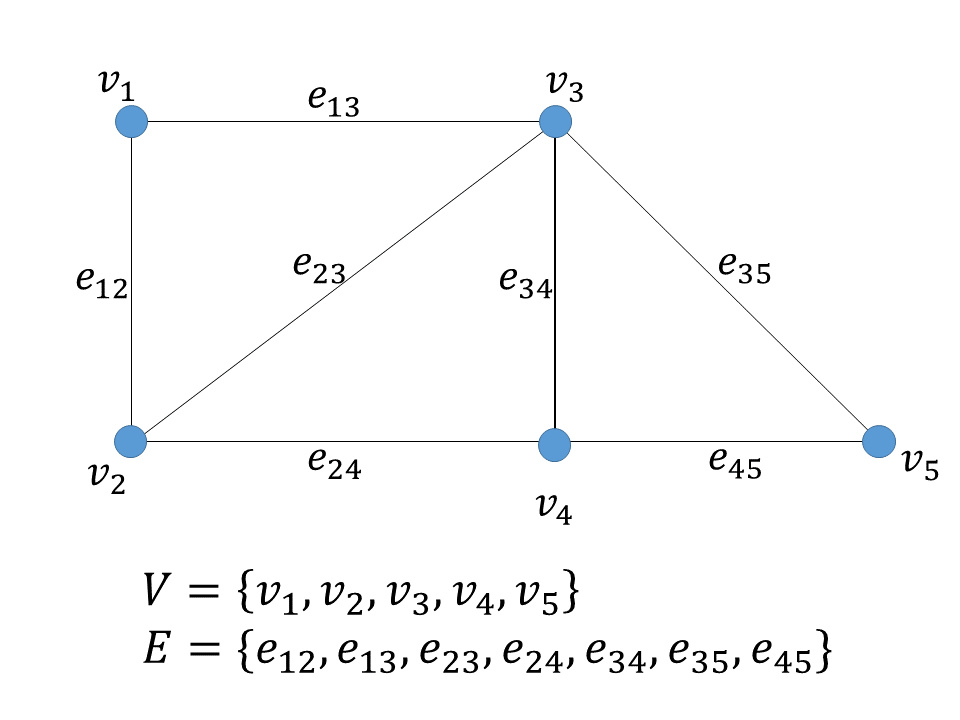
\includegraphics[width = 10cm]{graph1.png}
		\caption{A graph $G = (V, E)$\label{fig:graph}}
	\end{center}
\end{figure}

A \textbf{complete graph\index{complete graph}} is a simple undirected graph in which every pair of vertices is connected by an edge.
The complete graph with $n$ vertices is often denoted by $K_n$ (Figure \ref{fig:complete}). 
It is clear that a complete graph $K_n$ has $n(n-1)/2$ edges.

\begin{figure}[h!]
	\begin{center}
		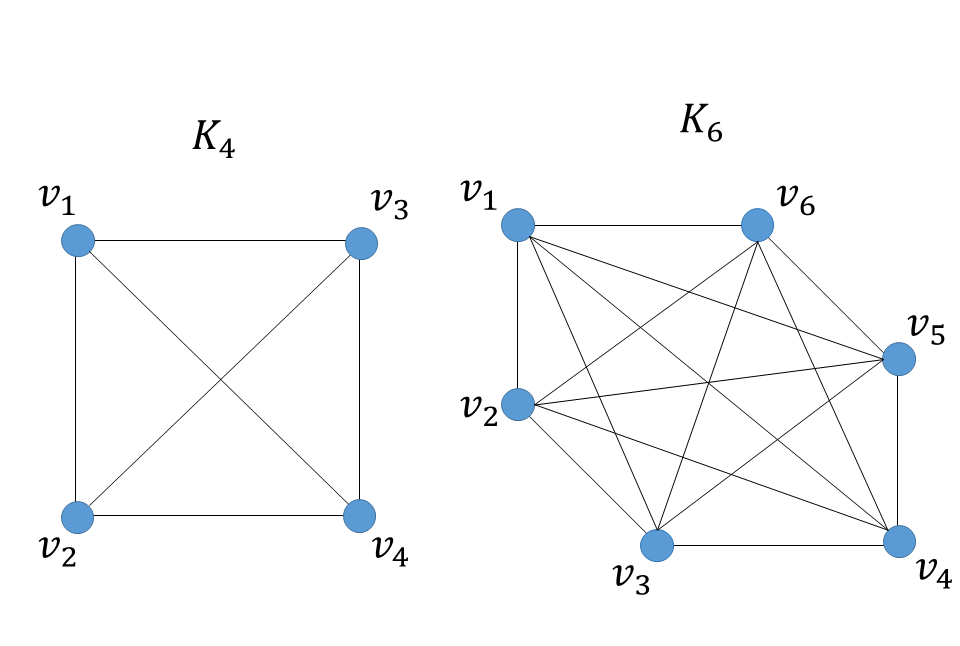
\includegraphics[width = 10cm]{complete.png}
		\caption{Complete graphs\label{fig:complete}}
	\end{center}
\end{figure}

\section{Paths, Cycles and Connectivity}

For a graph $G = (V, E)$, a \textbf{walk\index{walk}} from $v_i$ to $v_t$ is a finite sequence of edges of the form $e_{ij}, e_{jk}, \ldots , e_{ls}, e_{st}$.
If the starting vertex and the ending vertex are same, i.e., $v_i = v_t$, we say that the walk is \textbf{closed\index{closed}}.
The number of edges included in a walk is called its \textbf{length\index{length}}.
A walk $e_{ij}, e_{jk}, \ldots , e_{ls}, e_{st}$ in which all the edges $\{e_{ij}, e_{jk}, \ldots , e_{ls}, e_{st}\}$ are distinct is called a \textbf{trail\index{trail}}.
In addition, a walk in which all the vertices $\{v_i, v_j, v_k, \ldots v_l, v_s, v_t\}$ are distinct (except, possibly, $v_i = v_t$) is a \textbf{path\index{path}}.
A closed path is called a \textbf{cycle\index{cycle}}.
For vertices $v_i$ and $v_j$, the \textbf{distance} from $v_i$ to $v_j$ is the length of the shortest path from $v_i$ to $v_j$.
When a graph is directed, there may exist one-way edges in the graph.
Therefore, in this case the distance from $v_i$ to $v_j$ does not generally coincide with that from $v_j$ to $v_i$.
\bigskip

We say that a graph is \textbf{connected\index{connected}} if there is a path between each pair of vertices, otherwise it is said to be disconnected (Figure \ref{fig:connected}).
When a graph is disconnected, it is possible that there is no path between a pair of vertices.
In this case, we set the distance between them to infinity.

\begin{figure}[h!]
	\begin{center}
		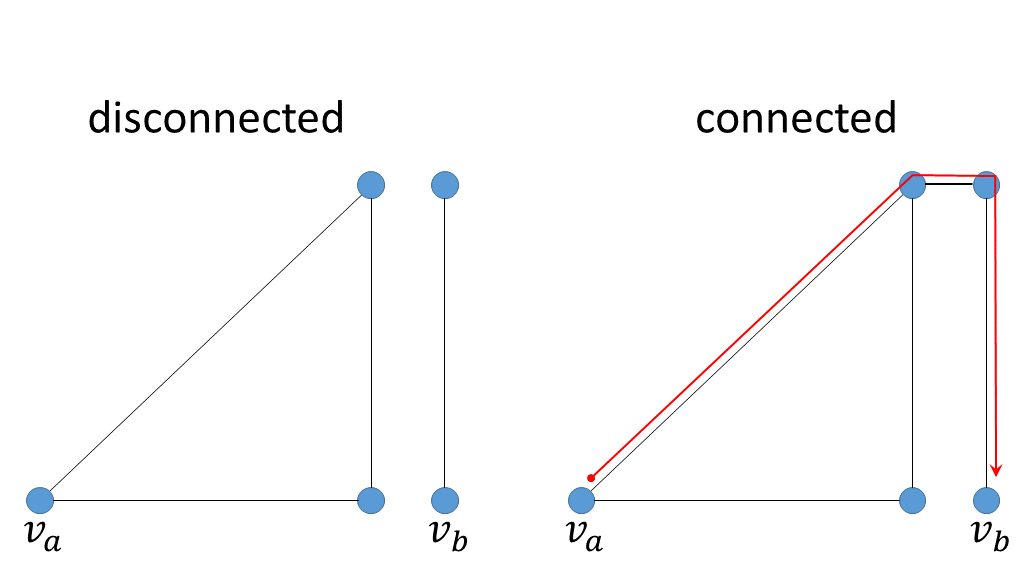
\includegraphics[width = 12cm]{connected.png}
		\caption{Connected/disconnected graph\label{fig:connected}}
	\end{center}
\end{figure}

The next result provides an easy-to-check sufficient condition for a graph to be connected.
\begin{proposition}
	Let a graph $G = (V, E)$ be a simple graph with $n \ge 2$ vertices. 
	If the number of edges in $G$ is larger than $(n-1)(n-2)/2$, then the graph is connected.
\end{proposition}

\begin{proof}
	We prove the result by contradiction.
	Suppose that $G$ is disconnected and is comprised of $k > 1$ connected graph components.
	It is clear that the maximum number of edges that $G$ can contain decreases as $k$ increases.
	Thus, it is sufficient to consider the case $k = 2$.
	Let $G_1$ and $G_2$ be connected graphs with $n_1$ and $n_2$ vertices, respectively, such that $G = G_1 \cup G_2$ ($n_1 + n_2 = n$).
	Here, note that, in order to attain the maximum number of edges, (without loss of generality) $G_1$ must be a single vertex without edges and $G_2$ must be a complete graph $K_{n-1}$.
	Then, since the number of edges in $K_{n-1}$ is equal to $(n-1)(n-2)/2$, the number of edges in $G$ is at most $(n-1)(n-2)/2$, which is a contradiction with the assumption.
	Thus, $G$ is connected.
\end{proof}

\section{Degree}

For a graph $G = (V, E)$, if there is an edge $e_{ij} \in E$ between $v_i$ and $v_j$, we say that $v_i$ and $v_j$ are \textbf{adjacent\index{adjacent}}.
In a complete graph, all pairs of vertices are adjacent.
When $v_i$ and $v_j$ are adjacent, we say that the vertices $v_i$ and  $v_j$ are \textbf{incident\index{incident}} with the edge $e_{ij}$.

\begin{figure}[h!]
	\begin{center}
		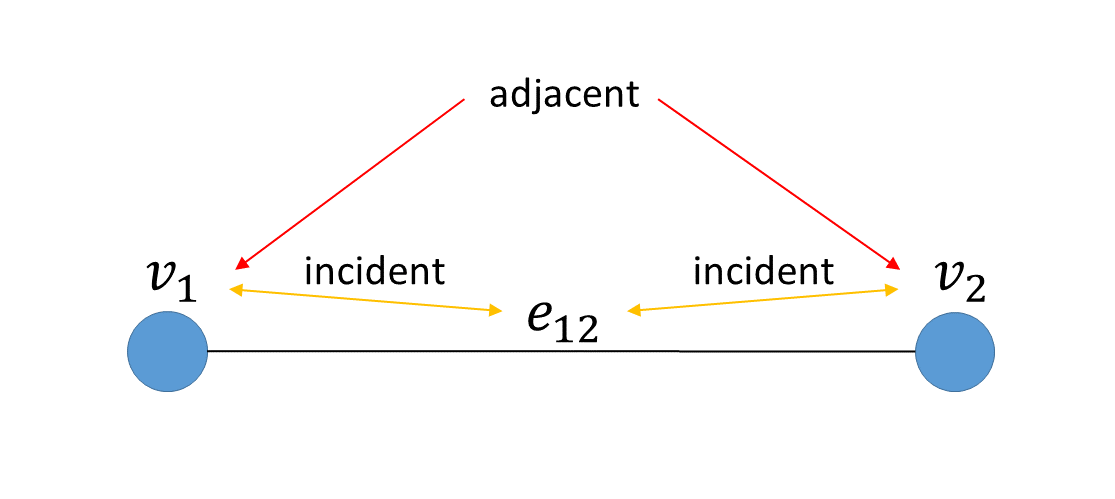
\includegraphics[width = 10cm]{adjacent.png}
		\caption{Adjacency and incidence\label{fig:adjacency}}
	\end{center}
\end{figure}

The \textbf{degree\index{degree}} of a vertex $v$ of a graph $G$ is the number of edges incident with $v$, which we denote as $d_G(v)$.
A loop is counted twice in $d_G(v)$.
A vertex of degree $d_G(v) = 0$ and $d_G(v) = 1$ are said to be \textbf{isolated vertex\index{isolated vertex}} and \textbf{end vertex\index{end vertex}} of $G$, respectively.
When the graph $G = V(V, E)$ is simple with no loops and multiple edges, the degree of a vertex $v_i \in V$ is equal to the number of vertices adjacent to $v_i$, namely,
\[
	d_G(v_i) = | \{v_j \in V : e_{ij}\in E\} |,
\]
where $| A |$ denotes the cardinality of set $A$.
For a complete graph $K_n$, the degrees of all vertices are equal to $n - 1$.

\begin{figure}[h!]
	\begin{center}
		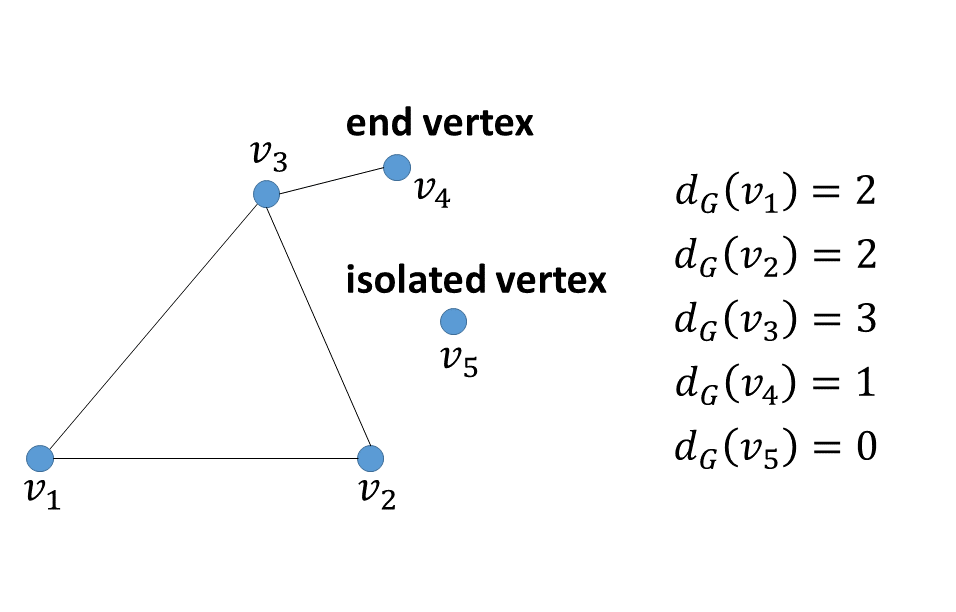
\includegraphics[width = 10cm]{degree.png}
		\caption{Degree\label{fig:degree}}
	\end{center}
\end{figure}

The next result is often referred to as the ``handshaking'' lemma:
\begin{proposition}[Handshaking]\label{prop:handshake}
	For any graph $G = (V, E)$, $\sum_{v \in V} d_G(v) = 2 | E |$.
	(The total number of hands shaken is twice the number of handshakes.)
\end{proposition}

\begin{proof}
	Let $\mathbf{1}(v \sim e)$ be an indicator that takes 1 if $v$ is incident with $e$ and 0 otherwise.
	Then, we can write $d_G(v) = \sum_{e \in E}\mathbf{1}(v \sim e)$.
	Note that each edge contributes 2 to the sum of degrees: $\sum_{v \in V}\mathbf{1}(v \sim e) = 2$ holds for each $e \in E$.
	Thus,
	\begin{align*}
		\sum_{v \in V} d_G(v) 
		& = \sum_{v \in V} \sum_{e \in E}\mathbf{1}(v \sim e) \\
		& = \sum_{e \in E} \;\; \underbrace{\sum_{v \in V} \mathbf{1}(v \sim e)}_{=2} = 2 |E|.
	\end{align*}
\end{proof}

As a corollary of the above result, we can easily show that the number of vertices of odd degree is even.

\section{Eulerian graph}

A connected graph $G$ is an \textbf{Eulerian graph\index{Eulerian graph}} if there exists a closed trail containing every edge of $G$.
Such a trail is called an \textbf{Eulerian trail\index{Eulerian trail}}.
In other words, an Eulerian graph is a graph that can be drawn unicursally without lifting one's pencil from the paper and without repeating any lines.

Then, the problem of K\"onigsberg bridges is equivalent to asking whether the lower-right graph in Figure \ref{fig:euler} has an Eulerian trail.
In 1736, Euler proved that if the degree of each vertex of $G$ is an even number, then $G$ has an Eulerian trail.
From this result, we can see that the upper graphs in Figure \ref{fig:euler} are Eulerian, and the lower graphs are not.

\begin{figure}[h!]
	\begin{center}
		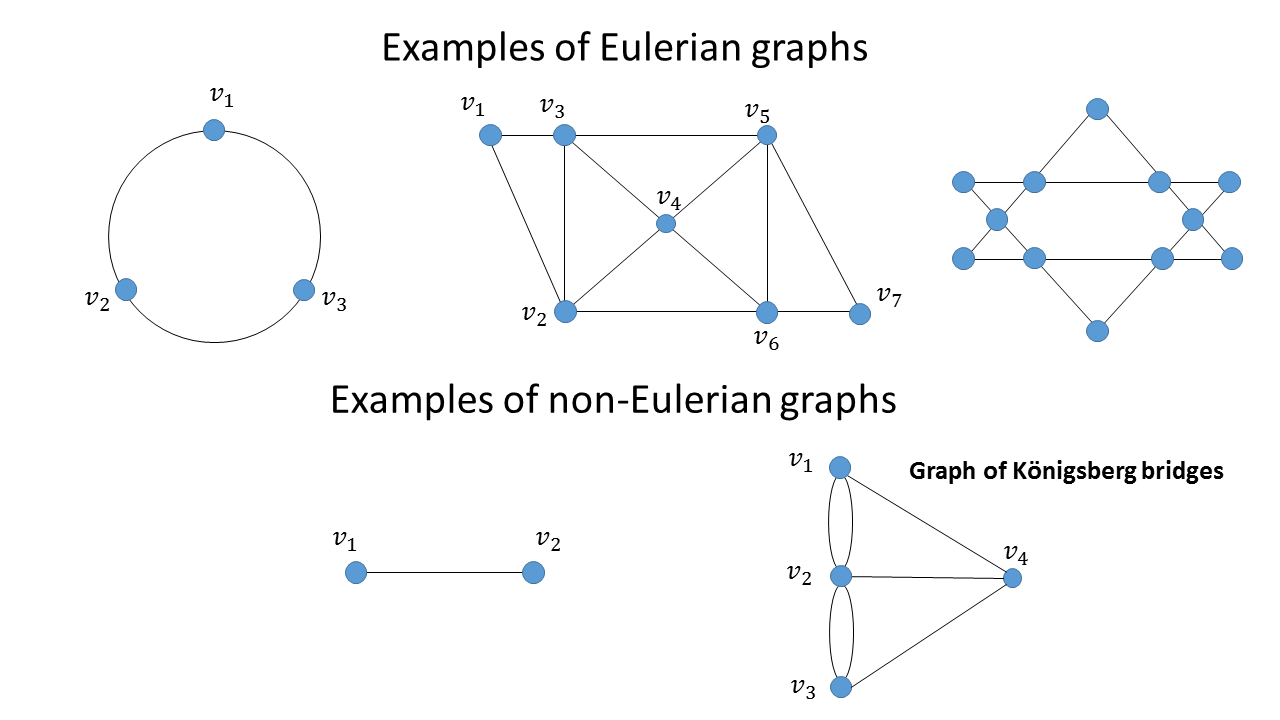
\includegraphics[width = 15cm]{graphs.png}
		\caption{Eulerian graphs and non-Eulerian graphs\label{fig:euler}}
	\end{center}
\end{figure}

Before providing the proof of this result, we prove the following useful lemma.
\begin{lemma}\label{lem:cycle}
	If $G$ is a graph in which the degree of each vertex is at least $2$, then $G$ contains a cycle (recall: cycle = closed path).
\end{lemma}

\begin{proof}
	If $G$ has loops or multiple edges, the result trivially holds.
	Then, suppose that $G$ is a simple graph.
	Let $v$ be any vertex of $G$, and construct a walk starting from $v$, say $v \to v_1 \to v_2 \to \cdots $, by choosing $v_{i+1}$ such that $v_{i+1}$ is adjacent to $v_i$ and $v_{i+1} \neq v_{i-1}$.
	The existence of such walk is guaranteed by the simplicity of $G$ and the assumption made.
	Since the number of vertices if finite, we must eventually choose a vertex that has been chosen before.
	Letting $v_k$ be the first such vertex, the walk contains a cycle starting from $v_k$.
\end{proof}

Now, we state Euler's (1736) result formally as follows:
\begin{theorem}
	A connected graph $G = (V,E)$ is Eulerian if and only if the degree of each vertex of $G$ is even.
\end{theorem}

\begin{proof}
	(Eulerian $\Rightarrow$ the degrees of the vertices are even.) Suppose that $P$ is an Eulerian trail of $G$.
	Whenever $P$ passes through a vertex, there is a contribution of 2 to the degree of that vertex.
	Since each edge appears exactly once in $P$, the degree of each vertex must be even.
	\bigskip
	
	(The degrees of the vertices are even $\Rightarrow$ Eulerian.) We prove the result by induction with respect to $q = |E|$.
	If $q \le 2$, the result trivially holds.
	Then, suppose that $q > 2$ and the result holds for any connected graph $G' = (V', E')$ with $|E'| \le q - 1$.
	Since the degrees of the vertices of $G$ are at least 2, by Lemma \ref{lem:cycle}, we can construct a cycle $C: v_1 \to v_2 \to \cdots \to v_1$ in $G$.
	Let $G_1 = (V_1, E_1)$ be a graph obtained by eliminating the edges in $C$ from $G$.
	Since $|E_1| \le q - 1$, $G_1$ is Eulerian by assumption.
	Here, we can choose a vertex $v^* \in V_1$ which is included in the cycle $C$. 
	Noting that an Eulerian trail can be started at any vertex and it will end at the same vertex, we can construct an Eulerian trail of $G_1$ starting and ending at $v^*$, say $P^*$.
	Then, the cycle $v_1 \to v_2 \to \cdots \to \underbrace{v^* \to \cdots \to v^*}_{P^*} \to \cdots \to v_1$ is an Eulerian trail of $G$.
\end{proof}
\section{Adjacency matrix}\label{sec:adjacency}

For a graph $G = (V, E)$ with $n$ vertices $\{v_1, \ldots, v_n\}$, its \textbf{adjacency matrix\index{adjacency matrix}} $A_n = (a_{i,j})$ is the $n \times n$ matrix whose $(i,j)$-th element is the number of edges joining $v_i$ and $v_j$.
If $G$ has no loops, the diagonal elements of $A_n$ are zero.
Further, if $G$ has no multiple edges, each $(i,j)$-th element of $A_n$ is an indicator whether $v_i$ is adjacent to $v_j$ or not.
Adjacency matrix of an undirected graph is symmetric, while that of an directed graph can be asymmetric (Figure \ref{fig:adjmat}).
The adjacency matrix $A_n$ contains all the information about the graph $G$.

\begin{figure}[h!]
	\begin{center}
		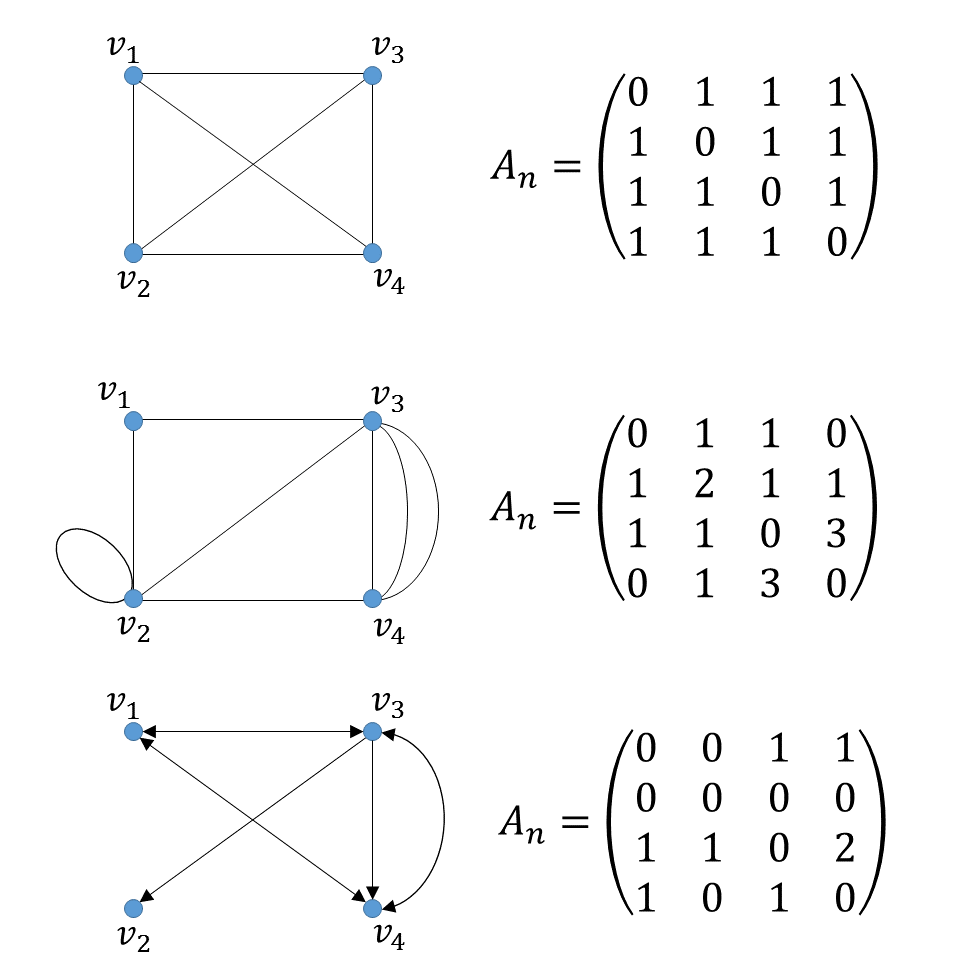
\includegraphics[width = 12cm]{adjmat.png}
		\caption{Adjacency matrix\label{fig:adjmat}}
	\end{center}
\end{figure}

\subsection*{Some useful properties of adjacency matrix}

\begin{enumerate}
	\item Using the adjacency matrix, the degree of vertex $v_i$ can be calculated as
	\[
		d_G(v_i) = \sum_{j = 1}^n a_{i,j}
	\]
	which is the $i$-th row sum of $A_n$.
	In the case of directed graph, the $i$-th row sum of $A_n$ corresponds to the ``out-degree'' of $v_i$.
	By Proposition \ref{prop:handshake}, it follows that the total number of edges is equal to one-half of the sum of all entries of $A_n$.
	\item For a non-negative integer $\ell$, the $(i,j)$-th element of $A_n^\ell$ equals to the number of walks of length $\ell$ from $v_i$ to $v_j$. (We define $A_n^0$ to be the identity matrix $I_n$.)
	Recall that $a_{ik}$ tells us the number of edges from $v_i$ to $v_k$.
	Hence, the number of walks of length 2 from $v_i$ to $v_j$ passing through $v_k$ is obtained by $a_{ik}a_{kj}$, and the total number of such walks is $\sum_{k = 1}^n a_{ik}a_{kj} = (A_n^2)_{i,j}$.

	\begin{figure}[h!]
		\begin{center}
			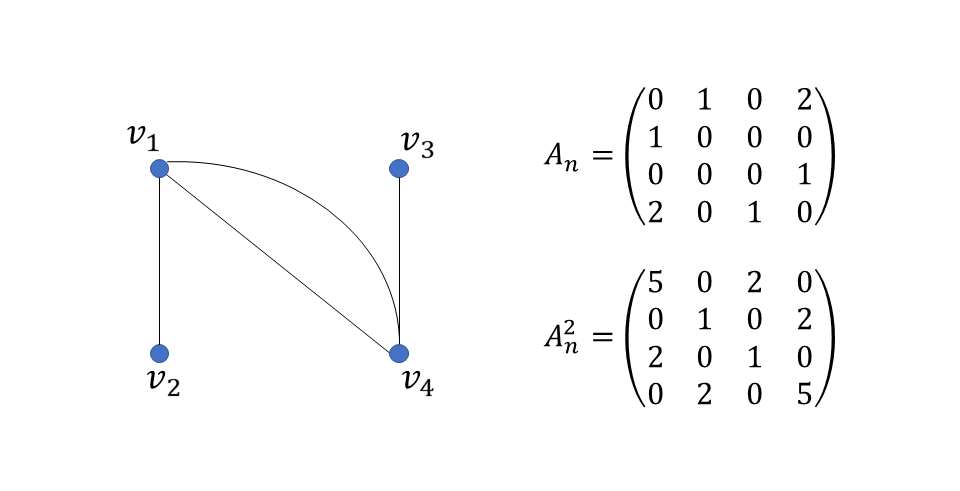
\includegraphics[width = 12cm]{nwalks.png}
			\caption{Number of walks\label{fig:nwalks}}
		\end{center}
	\end{figure}

	By using this property, one can easily find the shortest path length between a given pair of vertices.
	For example, suppose that $ (A_n)_{i,j} =  (A_n^2)_{i,j} = \cdots =  (A_n^{\ell - 1})_{i,j} = 0$ and $(A_n^\ell)_{i,j} > 0$. 
	Then, the shortest path length between $v_i$ and $v_j$ is $\ell$.
\end{enumerate}

\section{Centrality in networks}
In empirical network analysis, we often want to identify which agents (vertices/nodes) are most ``central''.
The definition of ``centrality'' varies by contexts and purposes.

The most basic centrality measure is the \textbf{degree centrality\index{degree centrality}} of a vertex $v$, which is simply defined as the degree of $v$, $d_G(v)$.
The degree centrality is based on an idea that a person who has many connections is the most important person.
For example, see the graph in Figure \ref{fig:center}.
For this graph, the most central vertices in terms of the degree centrality are $v_3$ and $v_5$.
However, in this example, one might consider that $v_4$ is more central than $v_3$ and $v_5$.

Here, let us denote the distance (i.e., the length of the shortest path) between the vertices $v_i$ and $v_j$ by $\Delta(v_i, v_j)$.
The \textbf{eccentricity\index{eccentricity}} $e(v)$ of a node $v$ in a connected graph $G = (V, E)$ is the maximum distance between $v$ and $u \in V$, that is
\[
	e(v) = \max_{u \in V} \Delta(v, u).
\]
When $G$ is not connected, we define $e(v) = \infty$ for all $v$.
Then, the reciprocal of the eccentricity value can be also used as a measure of centrality.
Based on this centrality measure, the most central vertex in the graph in Figure \ref{fig:center} is $v_4$.

More sophisticated centrality measure can be constructed based on the accessibility to other vertices, including not only adjacent vertices but also those that are not adjacent in the graph. 
Here, recall that the $(i,j)$-th element of the $\ell$-th power of the adjacency matrix $A_n^\ell$ represents the number of walks of length $\ell$ from $v_i$ to $v_j$, where $n$ is the number of vertices in the graph.
Thus, letting $\mathbf{1}_n$ be the vector of ones of length $n$, the $i$-th element of $A_n^\ell \mathbf{1}_n$ is equal to:
\[
	(A_n^\ell \mathbf{1}_n)_i = \text{the number of vertices reachable from $v_i$ by length-$\ell$ walk.}
\]
Let $\beta \in (0,1)$ be an ``propagation factor'' for an increase of the length.
(For example, one may interpret $\beta$ as the magnitude of peer effects; or, for another example, the rate of infection of a disease to neighboring residents.)
Then, we can consider the $i$-th element of $C_n(\beta)$, where
\[
	C_n(\beta) = \left( \sum_{\ell = 0}^\infty \beta^\ell A_n^\ell \right) \mathbf{1}_n,
\]
as the $i$-th centrality value, which is called the \textbf{Bonacich centrality\index{Bonacich centrality}}.

\begin{figure}[h!]
	\begin{center}
		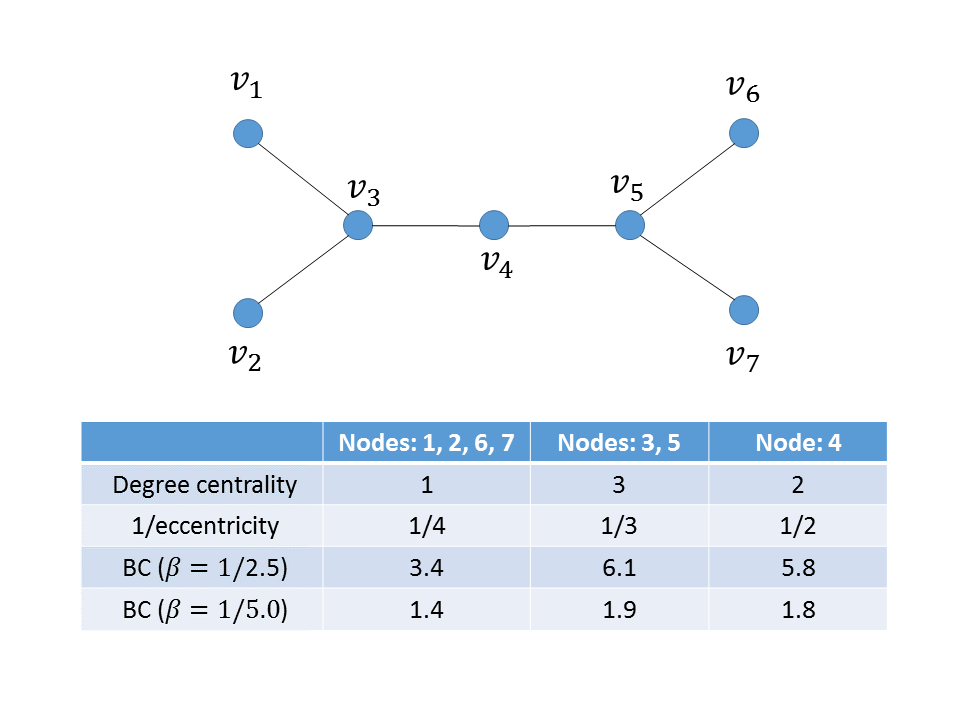
\includegraphics[width = 14cm]{central.png}
		\caption{Centrality measures\label{fig:center}}
	\end{center}
\end{figure}

In the third and the fourth row of the table in Figure \ref{fig:center}, we report the Bonacich centrality of each vertex with $\beta = 1/2.5$ and $\beta = 1/5$, respectively.
As we can see, in terms of Bonacich centrality, the centrality of the vertices 3, 4 and 5 becomes more (less) prominent if the propagation factor $\beta$ is large (small).

It is important to note that a higher-order matrix polynomial $\beta^\ell A_n^\ell$ can quickly diverge to infinity for some choice of $\beta$.
When $\beta$ is appropriately chosen so that $C_n(\beta)$ exists, using the Neumann series formula, it can be exactly obtained by
\[
C_n(\beta) = \left(I_n - \beta A_n \right)^{-1}\mathbf{1}_n,
\]
where $I_n$ is the $n \times n$ identity matrix (see Appendix \ref{sec:neumann} for details).
An easy-to-check sufficient condition for the existence of $C_n(\beta)$ is that $\beta \cdot \max_{v \in V}d_G(v) < 1$.

In the literature on network games, the Bonacich centrality has an important role in identifying the \textit{key player}, the player who, once removed from the network, causes the most significant impact on the aggregate outcome such as total welfare of the network (see, e.g., \cite{ballester2006s}).

%%%%%%%%%%%%%%%%%%%%%%%%%%%%%%%%%%%%%%%

\chapter{Supplementary Mathematical Notes}
\section{Some supplementary results in probability theory.}
\begin{lemma}\label{lem:prodconv}
Let $X_n \in \mathbb{R}$ and $Y_n \in \mathbb{R}$ be sequences of random variables such that $X_n \overset{p}{\to} \bar X$ and $Y_n \overset{p}{\to} \bar Y$, respectively, where both $\bar X$ and $\bar Y$ are finite.
Then, it holds that $X_n Y_n \overset{p}{\to} \bar X \bar Y$.
\end{lemma}

\begin{proof}
	By the triangle inequality,
	\begin{align*}
	|X_n Y_n - \bar X \bar Y|
	& = |X_n Y_n - \bar X Y_n + \bar X Y_n - \bar X \bar Y| \\
	& \le |X_n Y_n - \bar X Y_n| + |\bar X Y_n - \bar X \bar Y| \\
	& = |Y_n| \cdot |X_n - \bar X| + |\bar X |\cdot | Y_n - \bar Y|. 
	\end{align*}
	The second term on the right-hand side clearly converges to zero in probability.
	For the first term, note that $|Y_n|$ is not necessarily finite for some $n$.
	Let $\kappa > 0$ and $\eta > 0$ be positive numbers.
	 \begin{align*}
	\Pr(|Y_n| \cdot |X_n - \bar X| > \kappa) 
	& = \Pr(|Y_n| \cdot |X_n - \bar X| > \kappa, |Y_n| \le 1/\eta) +	\Pr(|Y_n| \cdot |X_n - \bar X| > \kappa, |Y_n| > 1/\eta) \\
	& \le \Pr(|X_n - \bar X| > \kappa \eta) +	\Pr(|Y_n| > 1/\eta) \\
	& \le \Pr(|X_n - \bar X| > \kappa \eta) +	\Pr(|\bar Y| > 1/(2\eta)) + \Pr(|Y_n - \bar Y| > 1/(2\eta)).
	 \end{align*}
	By choosing sufficiently small $\eta$, the terms on the right-hand side all converge to zero in probability by assumption.
	Thus, we have 
	 \[
	 \lim_{n\to\infty} \Pr(|Y_n| \cdot |X_n - \bar X| > \kappa) = 0.
	 \]
	 Since ths choice of $\kappa$ is arbitrary, this gives the desired result.
\end{proof}

\begin{lemma}[Slutsky's theorem]\label{lem:slutsky}
	Let $X_n \in \mathbb{R}$ and $Y_n \in \mathbb{R}$ be sequences of random variables such that $X_n \overset{d}{\to} \bar X$ and $Y_n \overset{p}{\to} c$, respectively.
	Then,
	\begin{align*}
	\mathrm{(i)} & \;\; X_n + Y_n \overset{d}{\to} \bar X + c,\\
	\mathrm{(ii)} & \;\; X_n Y_n \overset{d}{\to} c \bar X.
	\end{align*}
	More generally, $g(X_n, Y_n) \overset{d}{\to} g(\bar X, c)$ holds for any continuous function $g(\cdot, \cdot)$. 
\end{lemma}
The proof is omitted (see, e.g., Lemma 2.8 in \cite{van2000asymptotic}).

\begin{lemma}[Jensen's inequality]\label{lem:Jensen}
	 Let $X \in \mbb{R}$ be a random variable and $\varphi(\cdot)$ be a convex function.
	 Then,
	\[
		\E[\varphi(X)] \ge \varphi(\E[X]). 
	\]
	If $\varphi(\cdot)$ is concave, then
	\[
		\E[\varphi(X)] \le \varphi(\E[X]). 
	\]
\end{lemma}

\begin{proof}
	Suppose that $\varphi(\cdot)$ is a convex function.
	Let $L(x) = a + bx$ be a straight line which is tangent to $\varphi(x)$ at $x = \E[X]$.
	Since $\varphi(\cdot)$ is convex, for all $x$, $\varphi(x) \ge L(x)$.
	Thus,
	\begin{align*}
	\E[\varphi(X)] 
	& \ge \E[L(X)] = \E[a + bX] = a + b \E[X] = L(\E[X]) =  \varphi(\E[X]).
	\end{align*}
	\begin{center}
		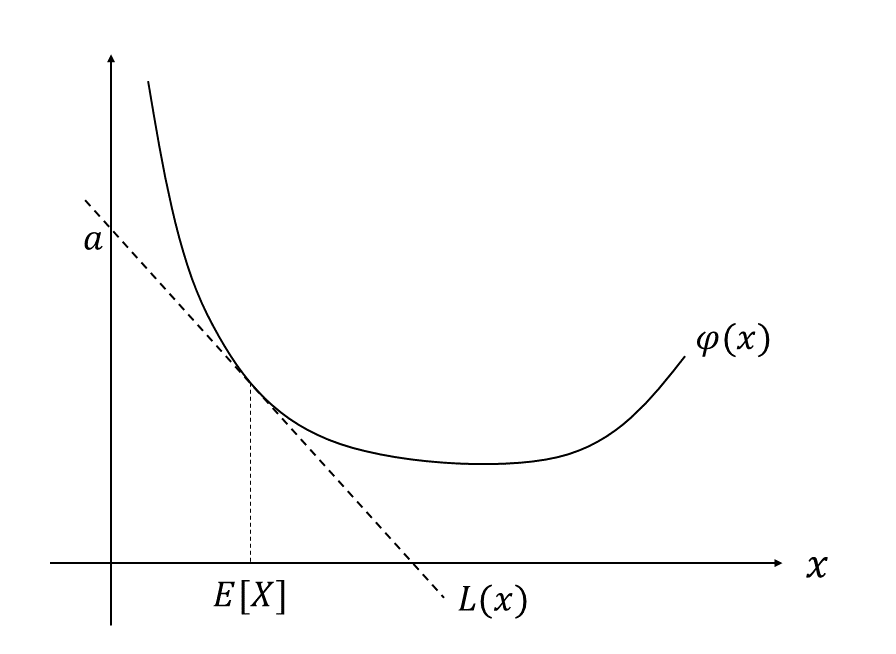
\includegraphics[width = 10cm]{jensen.png}
	\end{center}

\end{proof}

\begin{lemma}[Cauchy-Schwarz inequality]\label{lem:CS}
	For any random variables $X \in \mbb{R}$ and $Y \in \mbb{R}$, we have
	\[
	\left| \E[XY] \right| \le \sqrt{\E[X^2]} \sqrt{\E[Y^2]}. 
	\]
\end{lemma}

\begin{proof}
	When either $\E[X^2] = 0$ or $\E[Y^2] = 0$ is true, the result follows trivially with equality.
	Thus, we may consider the case where $\E[X^2], \E[Y^2] > 0$.
	Let us define $W = (X - c Y)^2$ for some constant $c$.
	Since $W$ is a non-negative random variable, we must have
	\begin{align*}
		0 
		& \le \E[W] \\
		& = \E[X^2] - 2c\E[XY] + c^2 \E[Y^2].
	\end{align*}
	Further, if we choose $c = \frac{\E[XY]}{\E[Y^2]}$, we have
	\[
	 	\E[X^2] - 2c\E[XY] + c^2 \E[Y^2] = \E[X^2] - \frac{\E[XY]^2}{\E[Y^2]}.
	\]
	Combining these results yields the desired result.
\end{proof}
%%%%%%%%%%%%%%%%%%%%%%%%%%%%%%%%%%%%%%%
\section{Neumann series expansion}\label{sec:neumann}
Let $A = (a_{i,j})$ be a matrix of finite-dimension $n \times m$.\footnote{
	This is just for simplicity.
	In general, we can consider a linear operator $A$ on an infinite dimensional Banach space.
}
We use $||A||_\infty$ to denote its infinity-norm: $||A||_\infty \equiv \max_{1 \le i \le n}\sum_{j = 1}^m |a_{i,j}|$.

\begin{lemma}
	The infinity norm is sub-multiplicative.
	That is, for matrices $\underset{n \times m}{A} = (a_{i,j})$ and $\underset{m \times p}{B} = (b_{j,k})$, $||A B ||_\infty \le ||A||_\infty ||B||_\infty$ holds.
\end{lemma}

\begin{proof}
	\begin{align*}
	||A B ||_\infty
	& = \max_{1 \le i \le n}\sum_{k = 1}^p \left| \sum_{j = 1}^m a_{i,j} b_{j,k} \right| \\
	& \le \max_{1 \le i \le n}\sum_{k = 1}^p \sum_{j = 1}^m | a_{i,j}| \cdot |b_{j,k}| \\
	& =\max_{1 \le i \le n} \sum_{j = 1}^m | a_{i,j}| \sum_{k = 1}^p |b_{j,k}| \\
	& \le \max_{1 \le i \le n} \sum_{j = 1}^m | a_{i,j}| \max_{1 \le j \le m} \sum_{k = 1}^p |b_{j,k}| = ||A ||_\infty ||B||_\infty.
	\end{align*}
\end{proof}

The series of matrices $\sum_{t = 0}^\infty A^t$ is called the \textbf{Neumann series\index{Neumann series}}.
The Neumann series has the following important property:
\begin{lemma}[Neumann series expansion]\label{lem:neumann}
	Suppose that $A_n$ is an $n \times n$ symmetric matrix such that $||A_n||_\infty < 1$.
	Then, $I_n - A_n$ is nonsingular, and it holds that $(I_n - A_n)^{-1} = \sum_{t = 0}^\infty A_n^t$.
\end{lemma}

\begin{proof}
	The first part is an elementary result in matrix algebra. 
	For the second part, observe that, for some $t$,
	\begin{align*}
	(I_n - A_n) (I_n + A_n + A_n^2 + \cdots + A_n^t) 
	& =  (I_n + A_n + A_n^2 + \cdots + A_n^t)  -  \underbrace{A_n (I_n + A_n + A_n^2 + \cdots + A_n^t) }_{A_n + A_n^2 + \cdots + A_n^{t+1}} \\
	& = I_n - A_n^{t+1}.
	\end{align*}
	Multiplying both sides by $(I_n - A_n)^{-1}$ yields
	\begin{align*}
	& (I_n + A_n + A_n^2 + \cdots + A_n^t)  =   (I_n - A_n)^{-1} - (I_n - A_n)^{-1}A_n^{t+1}, \\
	& \text{and thus } (I_n - A_n)^{-1} - (I_n + A_n + A_n^2 + \cdots + A_n^t) =  (I_n - A_n)^{-1}A_n^{t+1}.
	\end{align*}
	Since the infinity norm is sub-multiplicative, noting that $||A_n||_\infty < 1$ by assumption,
	\begin{align*}
	|| (I_n - A_n)^{-1} - (I_n + A_n + A_n^2 + \cdots + A_n^t)||_\infty 
	& =  ||(I_n - A_n)^{-1}A_n^{t+1}||_\infty \\
	& \le  ||(I_n - A_n)^{-1}||_\infty ||A_n^{t+1}||_\infty \\
	& \le  ||(I_n - A_n)^{-1}||_\infty ||A_n||^{t+1}_\infty \to 0
	\end{align*}
	as $t \to \infty$.
\end{proof}

\section{Expectation of a truncated random variable}\label{sec:truncate}

Let $X$ be a continuous random variable with its probability distribution function $F(\cdot)$ and density function $f(\cdot)$.
Further, let $a$ be a constant.
Then, the conditional distribution of $X$ given that $X \leq a$ is obtained by
\begin{align*}
F(x \mid X \leq a)
& = \Pr(X \leq x \mid X \leq a)\\
& = \frac{\Pr(X \leq \min\{x, a\})}{\Pr(X \leq a)} = \left\{\begin{array}{cl}
1 & \text{ if $x \geq a$} \\ 
\frac{F(x)}{F(a)} & \text{ if $x < a$}
\end{array}	\right. .
\end{align*}
By differentiating the both sides with respect to $x$, the conditional density of $X$ given that $X \leq a$ is given by
\begin{align*}
f(x \mid X \leq a) = \left\{\begin{array}{cl}
0 & \text{ if $x \geq a$} \\ 
\frac{f(x)}{F(a)} & \text{ if $x < a$}
\end{array}	\right. .
\end{align*}
Thus, the expectation of $X$ conditional on $X \leq a$ is
\begin{align*}
\E[X \mid X \leq a] 
& = \int_{-\infty}^{\infty} x f(x \mid X \leq a) \mrm{d}x \\
& = \frac{\int_{-\infty}^a x f(x) \mrm{d}x}{F(a)}.
\end{align*}
By analogous arguments, we can show that the expectation of $X$ conditional on $X > a$ is obtained by
\begin{align*}
\E[X \mid X > a] 
& = \int_{-\infty}^{\infty} x f(x \mid X > a) \mrm{d}x \\
& = \frac{\int_a^\infty x f(x) \mrm{d}x}{1 - F(a)}.
\end{align*}

\section{The inverse of a partitioned matrix}
Consider a partitioned matrix
\[
	A = \left(\begin{array}{cc}
	A_{11} & A_{12} \\
	A_{21} & A_{22}
\end{array}	\right).
\]
Then, the inverse of $A$ is given by
\begin{align}\label{eq:inverse}
	A^{-1} = \left(\begin{array}{cc}
	(A_{11} - A_{12}A_{22}^{-1}A_{21})^{-1} & -(A_{11} - A_{12}A_{22}^{-1}A_{21})^{-1}A_{12}A_{22}^{-1} \\
	-(A_{22} - A_{21}A_{11}^{-1}A_{12})^{-1}A_{21}A_{11}^{-1} & (A_{22} - A_{21}A_{11}^{-1}A_{12})^{-1}
\end{array} \right).
\end{align}
\end{appendices}
\end{document}